\title{The canonical noise of an image}

Everybody knows about the {\bf random phase noise}: you keep the power
spectrum of an image and randomize its phases.  You obtain an image that has
the same ``texture'', but a completely randomized geometry.  You cannot
recognize any object.

%RUN_VERBATIMS sh &
\begin{verbatim}
fft 1 i/barb.png |plambda "0 rand join cexp cprod" |fft -1 - barb-rpn.png
\end{verbatim}
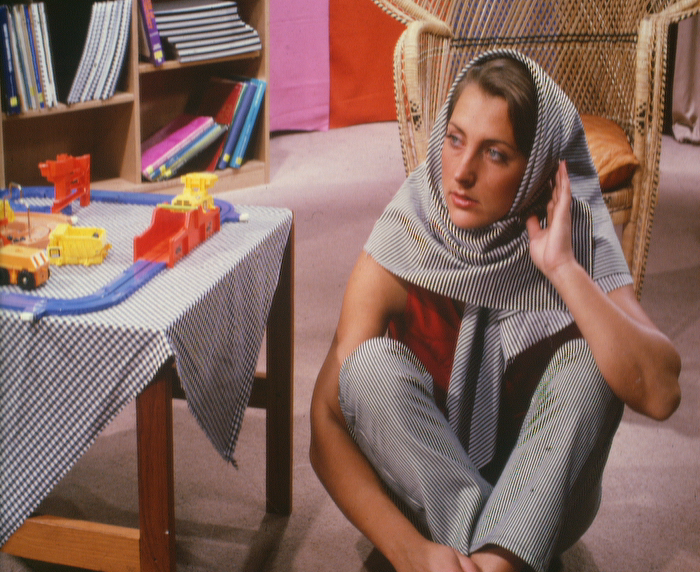
\includegraphics{i/barb.png}{\small\tt barb.png}\\

\includegraphics{barb-rpn.png}{\small\tt barb-rpn.png}

What happens if you do the opposite?  Keep the phases and randomize the
amplitudes?  Well, you lose all kind of texture but all the objects are
recognizable among the very spiky noise.

\begin{verbatim}
fft 1 i/barb.png|plambda "dup vnorm / randu *"|ifft|qauto -i -p 1 - barb-ran.png
\end{verbatim}
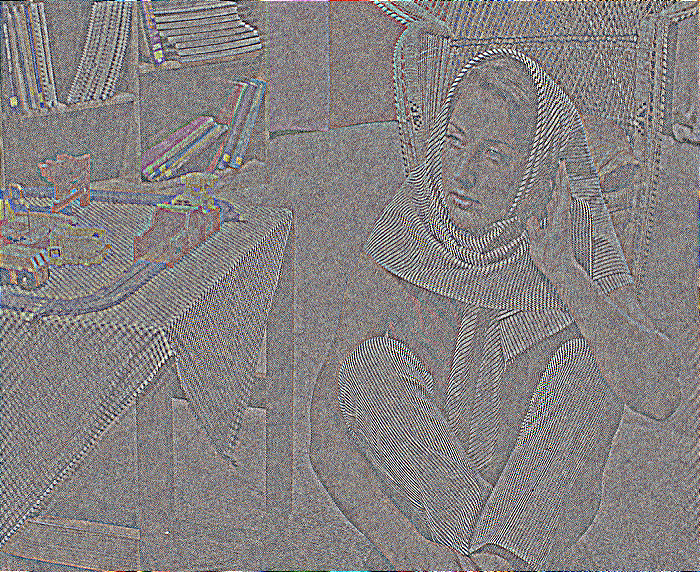
\includegraphics{barb-ran.png}{\small\tt barb-ran.png}


In fact, setting the amplitudes to uniform random is more or less the same
thing that setting them to a constant; the visual effect is very similar, but
with less noise.  This is called the~{\bf phase image}, because it is
obtained by throwing away all amplitude information (but not randomizing it)
and keeping only the phases.  It looks very different than the original
image, more or less like a laplacian.

\begin{verbatim}
fft 1 i/barb.png |plambda "dup vnorm /" |ifft |qauto -i -p 1 - barb-pha.png
\end{verbatim}
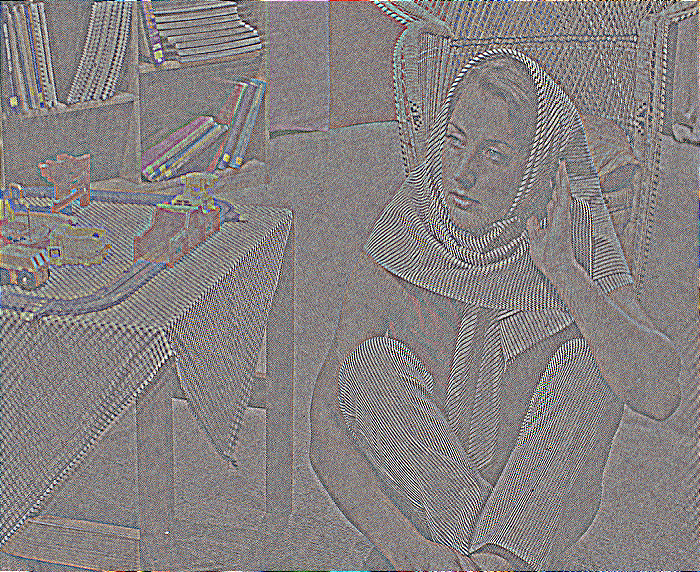
\includegraphics{barb-pha.png}{\small\tt barb-pha.png}


The phase image looks very strange because it has a flat spectrum, which is a
very unnatural spectrum to have.  Typically, the spectrum of images decays
with the inverse of the frequency.  Imposing this decay, instead of a flat
spectrum, we obtain the so-called {\em canonical image}:

\begin{verbatim}
fft 1 i/barb.png |plambda "dup vnorm / :R /" |ifft |qauto -i -p 1 - barb-can.png
\end{verbatim}
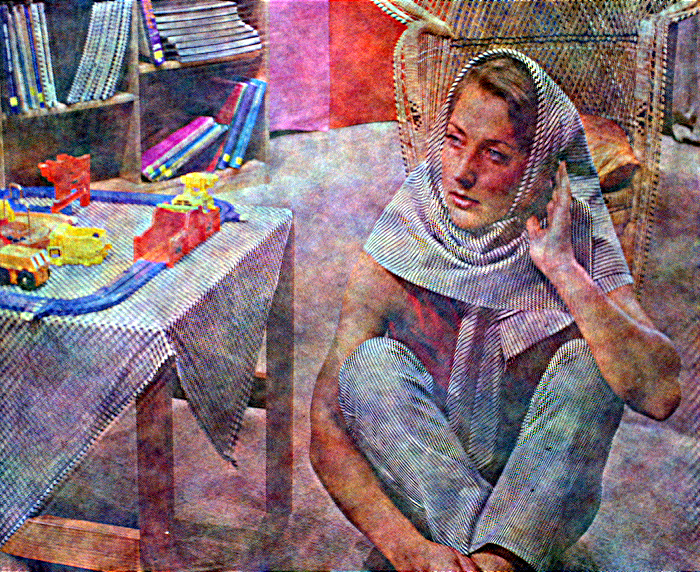
\includegraphics{barb-can.png}{\small\tt barb-can.png}


This image is eerily similar to the original.  It looks like a noisy version
of the original, but the noise is not white.  Interestingly, this noise has
been produced \emph{without any use of random numbers!}  We can call it the
{\bf canonical noise} of the image.  This works even with binary images:


\begin{verbatim}
fft <i/binbeck.png|plambda "dup vnorm / :R /" |ifft|qauto -p 1 - binbeck-can.png
\end{verbatim}

\includegraphics{i/binbeck.png}{\small\tt binbeck.png}\\
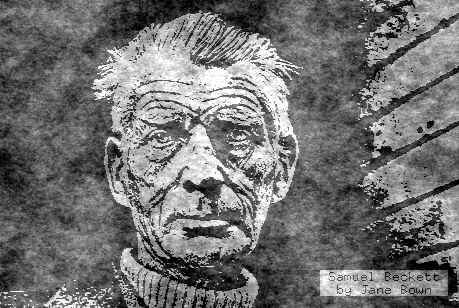
\includegraphics{binbeck-can.png}{\small\tt binbeck-can.png}



% vim:set tw=77 filetype=tex spell spelllang=en:
